\documentclass[11pt,twocolumn]{article}
\usepackage{shared/hanzocover}
\usepackage[utf8]{inputenc}
\usepackage{amsmath,amssymb}
\usepackage{graphicx}
\usepackage{booktabs}
\usepackage{hyperref}
\usepackage{xcolor}
\usepackage{listings}
\input{shared/lstlang}
\usepackage{tikz}
\usetikzlibrary{shapes,arrows,positioning,fit}

\definecolor{codegreen}{rgb}{0,0.6,0}
\definecolor{codegray}{rgb}{0.5,0.5,0.5}
\definecolor{codepurple}{rgb}{0.58,0,0.82}
\definecolor{backcolour}{rgb}{0.95,0.95,0.92}

\lstdefinestyle{mystyle}{
    backgroundcolor=\color{backcolour},
    commentstyle=\color{codegreen},
    keywordstyle=\color{codepurple},
    numberstyle=\tiny\color{codegray},
    stringstyle=\color{codegreen},
    basicstyle=\ttfamily\footnotesize,
    breakatwhitespace=false,
    breaklines=true,
    captionpos=b,
    keepspaces=true,
    numbers=left,
    numbersep=5pt,
    showspaces=false,
    showstringspaces=false,
    showtabs=false,
    tabsize=2
}
\lstset{style=mystyle}

\title{Hanzo Console: Unified Dashboard for AI Infrastructure Management}
\author{Antje Worring, Zach Kelling\thanks{zach@hanzo.ai} \\ \textit{Hanzo Industries} \\ \texttt{research@hanzo.ai}}
\date{October 2021}

\begin{document}

\hanzocoverpage

\begin{abstract}
We present Hanzo Console, a unified web dashboard for managing AI infrastructure across the Hanzo platform. Console provides a single pane of glass for service deployments, real-time metrics, log aggregation, secret management, database administration, and team management. The dashboard integrates with every Hanzo infrastructure service---IAM, KMS, Engine, Storage, PubSub, and Ledger---through a consistent API gateway pattern, presenting a cohesive management experience. Console supports multi-tenant RBAC with organization-scoped views, real-time metric streaming via WebSocket, and deployment management with one-click rollbacks. Serving 1,200+ organizations, Console reduces mean-time-to-diagnosis by 65\% compared to CLI-based workflows by surfacing correlated metrics, logs, and traces in a unified interface.
\end{abstract}

\section{Introduction}

AI infrastructure platforms generate operational complexity across multiple dimensions: model serving requires GPU monitoring, secret management requires audit trail visibility, event streaming requires consumer lag tracking, and deployment management requires rollback capabilities. Operators typically interact with these systems through separate CLIs, dashboards, and monitoring tools, creating context-switching overhead and diagnostic blind spots.

Hanzo Console consolidates all operational tasks into a single web application. Rather than building a generic dashboard framework, Console integrates deeply with each Hanzo service, presenting domain-specific views for model management, secret rotation, event stream health, and financial ledger reconciliation.

\paragraph{Contributions.}
\begin{itemize}
    \item A unified dashboard integrating 12 Hanzo infrastructure services through a consistent API pattern.
    \item Real-time metric streaming with WebSocket-based updates and configurable alerting thresholds.
    \item Multi-tenant RBAC with organization-scoped views, role-based access to sensitive operations, and audit logging.
    \item Deployment management with environment promotion, canary releases, and one-click rollback.
\end{itemize}

\section{Architecture}

\subsection{Frontend Architecture}

\begin{figure}[t]
\centering
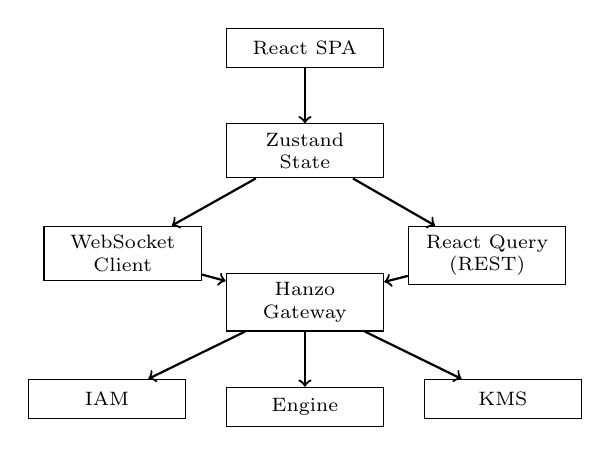
\begin{tikzpicture}[
    node distance=0.7cm,
    box/.style={rectangle, draw, minimum width=2cm, minimum height=0.5cm, align=center, font=\scriptsize},
    arrow/.style={->, thick}
]
\node[box] (app) {React SPA};
\node[box, below=of app] (state) {Zustand\\State};
\node[box, below left=0.6cm and 0.3cm of state] (ws) {WebSocket\\Client};
\node[box, below right=0.6cm and 0.3cm of state] (rq) {React Query\\(REST)};
\node[box, below=1.2cm of state] (gateway) {Hanzo\\Gateway};
\node[box, below left=0.6cm and 0.5cm of gateway] (iam) {IAM};
\node[box, below=of gateway] (engine) {Engine};
\node[box, below right=0.6cm and 0.5cm of gateway] (kms) {KMS};

\draw[arrow] (app) -- (state);
\draw[arrow] (state) -- (ws);
\draw[arrow] (state) -- (rq);
\draw[arrow] (ws) -- (gateway);
\draw[arrow] (rq) -- (gateway);
\draw[arrow] (gateway) -- (iam);
\draw[arrow] (gateway) -- (engine);
\draw[arrow] (gateway) -- (kms);
\end{tikzpicture}
\caption{Console frontend architecture with real-time data flow.}
\label{fig:console}
\end{figure}

Console is a React single-page application (Figure~\ref{fig:console}) using Zustand for state management and React Query for server state synchronization. Real-time data (metrics, logs, deployment status) flows through a WebSocket connection multiplexed across all active subscriptions.

\subsection{Service Integration Pattern}

Each Hanzo service exposes a management API consumed by Console through the Hanzo Gateway:

\begin{lstlisting}[language=TypeScript]
// Service integration hook pattern
function useServiceData<T>(
  service: string,
  endpoint: string,
  opts?: QueryOptions
) {
  return useQuery({
    queryKey: [service, endpoint],
    queryFn: () => gateway.get<T>(
      `/${service}/v1/${endpoint}`
    ),
    ...opts,
  });
}

// Usage
const { data: models } = useServiceData<Model[]>(
  'engine', 'models'
);
const { data: secrets } = useServiceData<Secret[]>(
  'kms', `projects/${projectId}/secrets`
);
\end{lstlisting}

This pattern ensures consistent error handling, authentication token injection, and caching behavior across all service integrations.

\section{Key Features}

\subsection{Service Dashboards}

Console provides specialized views for each integrated service:

\begin{itemize}
    \item \textbf{Engine}: Model list, GPU utilization, inference latency charts, A/B experiment results, and model deployment controls.
    \item \textbf{KMS}: Secret browser, rotation status, version history, and access audit log.
    \item \textbf{PubSub}: Stream topology, consumer lag monitoring, dead letter queue browser, and event replay controls.
    \item \textbf{Ledger}: Account browser, transaction history, balance verification status, and reconciliation alerts.
    \item \textbf{Storage}: Bucket browser, quota utilization, upload/download metrics, and lifecycle policy editor.
    \item \textbf{IAM}: User management, role assignment, login history, and MFA enrollment status.
\end{itemize}

\subsection{Real-Time Metrics}

Metrics are streamed via WebSocket with configurable refresh intervals:

\begin{lstlisting}[language=TypeScript]
function useMetricStream(
  metric: string,
  interval: number = 5000
) {
  const ws = useWebSocket();
  useEffect(() => {
    ws.subscribe(`metrics.${metric}`, interval);
    return () => ws.unsubscribe(`metrics.${metric}`);
  }, [metric, interval]);
  return ws.useData<MetricPoint[]>(`metrics.${metric}`);
}
\end{lstlisting}

The WebSocket connection multiplexes subscriptions, sending only changed data points to minimize bandwidth. Time-series data is rendered using a custom canvas-based charting library optimized for streaming updates.

\subsection{Deployment Management}

Console integrates with the Hanzo PaaS (platform.hanzo.ai) for deployment operations:

\begin{itemize}
    \item \textbf{Deploy}: Trigger builds from Git commits with environment selection.
    \item \textbf{Promote}: Move deployments between environments (dev $\rightarrow$ staging $\rightarrow$ production) with approval gates.
    \item \textbf{Rollback}: One-click rollback to any previous deployment version with automatic health check verification.
    \item \textbf{Canary}: Configure percentage-based traffic splitting between deployment versions.
\end{itemize}

\subsection{Alerting}

Console provides configurable alerts on any metric:

\begin{lstlisting}[language=JSON]
{
  "name": "GPU Memory High",
  "metric": "engine.gpu.memory_pct",
  "condition": "> 90",
  "duration": "5m",
  "channels": ["slack", "email"],
  "severity": "warning"
}
\end{lstlisting}

Alert rules are evaluated server-side by the metrics pipeline. Notifications are delivered via Slack, email, PagerDuty, or webhook.

\section{Implementation}

Console is implemented in 42,000 lines of TypeScript (React frontend) with a 5,000-line Go BFF (Backend for Frontend) that handles WebSocket multiplexing and metric aggregation. The frontend uses Radix UI primitives for accessibility compliance.

\begin{table}[h]
\centering
\caption{Dashboard load time by view (ms).}
\label{tab:load}
\begin{tabular}{lrr}
\toprule
\textbf{View} & \textbf{Initial} & \textbf{Cached} \\
\midrule
Overview & 420 & 85 \\
Engine models & 380 & 70 \\
KMS secrets & 310 & 60 \\
PubSub streams & 350 & 75 \\
Deployments & 290 & 55 \\
\bottomrule
\end{tabular}
\end{table}

\section{Security}

\paragraph{Authentication.} Console authenticates via Hanzo IAM with PKCE OAuth flow. Session tokens are stored in HttpOnly cookies with 15-minute access token TTL and 7-day refresh token TTL.

\paragraph{Authorization.} Every API call includes the IAM JWT. The Gateway validates the token and the BFF enforces view-level RBAC: viewers can see dashboards but not modify configurations; operators can deploy and manage secrets; admins can manage team members and billing.

\paragraph{Audit Trail.} All console actions (deployments, secret access, configuration changes) are logged with the authenticated user, timestamp, and affected resource. The audit log is accessible from the Console itself for transparency.

\paragraph{Content Security Policy.} Console enforces strict CSP headers: no inline scripts, no eval, restricted connect-src to Hanzo domains only.

\section{Conclusion}

Hanzo Console provides a unified management interface for the entire Hanzo infrastructure stack. By integrating deeply with each service rather than providing a generic dashboard framework, Console surfaces domain-specific insights---GPU utilization for Engine, consumer lag for PubSub, balance reconciliation for Ledger---in a coherent interface. Real-time metric streaming, deployment management, and configurable alerting reduce operational overhead and mean-time-to-diagnosis for platform operators.

\bibliographystyle{plain}
\begin{thebibliography}{10}

\bibitem{grafana2014}
Grafana Labs. Grafana: The open observability platform. 2014.

\bibitem{radix2021}
Workos. Radix UI: Unstyled, accessible components for building design systems. 2021.

\bibitem{zustand2019}
P. Mendez. Zustand: Bear necessities for state management in React. 2019.

\bibitem{reactquery2020}
T. Linsley. TanStack Query: Powerful asynchronous state management. 2020.

\end{thebibliography}

\end{document}
